% !TEX encoding = UTF-8 Unicode
\documentclass[convert={density=300,size=1000x700,outext=.png}]{standalone}
\usepackage{tikz}
% \usepackage[active,tightpage,psfixbb]{preview}
\usepackage{tipa}
% \PreviewEnvironment{pgfpicture}
% \setlength\PreviewBorder{2pt}

\begin{document}
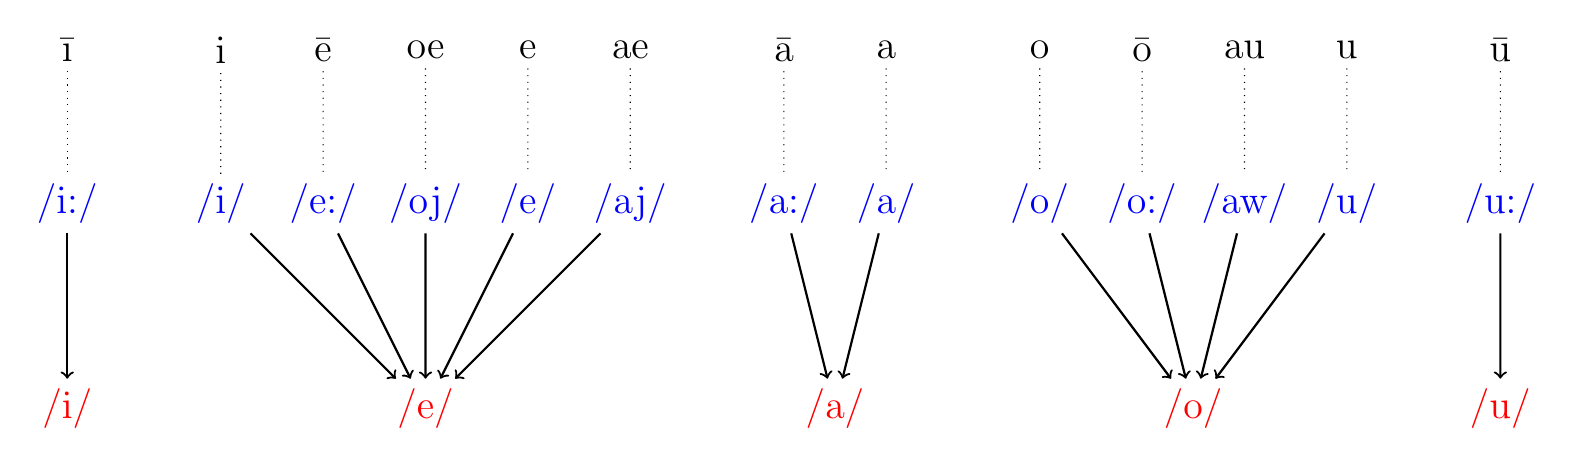
\begin{tikzpicture}[scale=.65]

% graphemes
\node [font=\Large] (a1) at (0,3) {\={\i}};

\node [font=\Large] (a2) at (3,3) {i};
\node [font=\Large] (a3) at (5,3) {\={e}};
\node [font=\Large] (a4) at (7,3) {oe};
\node [font=\Large] (a5) at (9,3) {e};
\node [font=\Large] (a6) at (11,3) {ae};

\node [font=\Large] (a7) at (14,3) {\={a}};
\node [font=\Large] (a8) at (16,3) {a}; 

\node [font=\Large] (a9) at (19,3) {o};
\node [font=\Large] (a10) at (21,3) {\={o}};
\node [font=\Large] (a11) at (23,3) {au};
\node [font=\Large] (a12) at (25,3) {u};

\node [font=\Large] (a13) at (28,3) {\={u}};


% vowels 1
\node [font=\Large,blue] (b1) at (0,0) {\textipa{/i:/}};

\node [font=\Large,blue] (b2) at (3,0) {\textipa{/i/}};
\node [font=\Large,blue] (b3) at (5,0) {\textipa{/e:/}};
\node [font=\Large,blue] (b4) at (7,0) {\textipa{/oj/}};
\node [font=\Large,blue] (b5) at (9,0) {\textipa{/e/}};
\node [font=\Large,blue] (b6) at (11,0) {\textipa{/aj/}};

\node [font=\Large,blue] (b7) at (14,0) {\textipa{/a:/}};
\node [font=\Large,blue] (b8) at (16,0) {\textipa{/a/}}; 

\node [font=\Large,blue] (b9) at (19,0) {\textipa{/o/}};
\node [font=\Large,blue] (b10) at (21,0) {\textipa{/o:/}};
\node [font=\Large,blue] (b11) at (23,0) {\textipa{/aw/}};
\node [font=\Large,blue] (b12) at (25,0) {\textipa{/u/}};

\node [font=\Large,blue] (b13) at (28,0) {\textipa{/u:/}};


% lines 1
\draw [dotted] (a1) -- (b1);
\draw [dotted] (a2) -- (b2);
\draw [dotted] (a3) -- (b3);
\draw [dotted] (a4) -- (b4);
\draw [dotted] (a5) -- (b5);
\draw [dotted] (a6) -- (b6);
\draw [dotted] (a7) -- (b7);
\draw [dotted] (a8) -- (b8);
\draw [dotted] (a9) -- (b9);
\draw [dotted] (a10) -- (b10);
\draw [dotted] (a11) -- (b11);
\draw [dotted] (a12) -- (b12);
\draw [dotted] (a13) -- (b13);



%vowels 2
\node [font=\Large,red] (c1) at (0,-4) {\textipa{/i/}};
\node [font=\Large,red] (c2) at (7,-4) {\textipa{/e/}};
\node [font=\Large,red] (c3) at (15,-4) {\textipa{/a/}};
\node [font=\Large,red] (c4) at (22,-4) {\textipa{/o/}};
\node [font=\Large,red] (c5) at (28,-4) {\textipa{/u/}};


% lines 2
\draw [->, thick] (b1) -- (c1);

\draw [->, thick] (b2) -- (c2);
\draw [->, thick] (b3) -- (c2);
\draw [->, thick] (b4) -- (c2);
\draw [->, thick] (b5) -- (c2);
\draw [->, thick] (b6) -- (c2);

\draw [->, thick] (b7) -- (c3);
\draw [->, thick] (b8) -- (c3);

\draw [->, thick] (b9) -- (c4);
\draw [->, thick] (b10) -- (c4);
\draw [->, thick] (b11) -- (c4);
\draw [->, thick] (b12) -- (c4);

\draw [->, thick] (b13) -- (c5);


\end{tikzpicture}
\end{document}